
\documentclass[british,11pt,a4paper]{article}
\usepackage[british]{babel}
\usepackage[margin=0.75in, bottom=0.75in, top=0.75in, footskip=0.25in]{geometry}
\usepackage[titletoc]{appendix}
\usepackage{fancyhdr}
\usepackage{mathtools}
\usepackage[numbers]{natbib}
\usepackage{pgfplotstable,filecontents}
\usepackage{hyperref}
\usepackage{booktabs}
\usepackage{wrapfig}
\usepackage{listings}
\usepackage{color}
\usepackage{graphicx}
\usepackage{siunitx}
\usepackage[parfill]{parskip}
\usepackage{tikz} % To generate the plot from csv
\usepackage{pgfplots}
\usepackage[normalem]{ulem}
\usepackage{longtable}
\usepackage{multirow}
\useunder{\uline}{\ul}{}
\usepackage{titlesec}

\setcounter{secnumdepth}{4}

\usepgfplotslibrary{statistics}

\pgfplotsset{compat=newest} % Allows to place the legend below plot
\usepgfplotslibrary{units} % Allows to enter the units nicely

\graphicspath{ {images/} }

\setcounter{secnumdepth}{2}
\setcounter{tocdepth}{2}
\renewcommand{\arraystretch}{1.2}
\renewcommand\thesection{\arabic{section}}
\renewcommand\thesubsection{\roman{subsection}.}
\renewcommand\thesubsubsection{}
\newcommand*{\Appendixautorefname}{appendix}
\pagestyle{fancy}
\fancyhf{}
\renewcommand{\headrulewidth}{0pt}
\lfoot{Exam no: Y0076159}
\cfoot{\thepage}
\lstset{
  columns=fixed,
  breaklines=true,
  basicstyle=\ttfamily\footnotesize
  }
% \titlespacing{\section}{1em}{\parskip}{-\parskip}
\titlespacing{\subsection}{0pt}{\parskip}{0.5em}
\titlespacing{\subsubsection}{0pt}{\parskip}{-\parskip}

\usepackage[nottoc]{tocbibind}
\usepackage{csvsimple}

\begin{document}
\title{PSEC Open Assessment}
\author{Exam no: Y0076159}
\date{\today}
\maketitle
\tableofcontents
\clearpage
\listoffigures
\listoftables
\clearpage

\section{Question 1 - Security risk management assessment}
\subsection{Purpose \& scope}
\label{subsec:purpose_scope}
The purpose of this report is to ensure the availability, integrity and safety of all stored and transmitted information within the SARTRE road train system. This is to ensure the availability of the system to users (which minimises a loss of turnover), the safety of the vehicles on the road (minimise legal liability / loss of turnover in the case of accidents), and most importantly the confidentiality of user data (minimise liability in the case of disclosure of customer information).

The sum of these ensures the compliance of the SARTRE project to IT statute and regulation. This will be ensured using a risk criteria evaluated against the ISO 27005  standard \cite{Iso2005-nn} for information security risk management. 

The report's scope is restricted to the entities owned by an implementation of the SARTRE project, including vehicles \& server hardware, software, personnel, business processes and use of technologies. 

\subsection{Risk evaluation criteria}
The risk evaluation criteria for this security assessment is defined by the following criteria, in order of decreasing importance.

The violation of IT statute and regulation (leading to the disclosure of customer information to cyber-criminals) is the paramount objective of this security analysis, as this could lead to theft or other forms of digital crime against users. 

Secondly, as the summary of policies for the SARTRE project \cite{Davila2013-cy} details that the liability of all vehicles in a road train falls on the lead vehicle, ensuring the safety of the system on the road is paramount to avoiding financial costs incurred due to accidents on the road. 

The availability of the system would greatly impact the financial feasibility of the project, as revenue depend on the usage of the system by users. Therefore maintaining the availability of the system ensures the availability of revenue for a larger period of time, and therefore the financial viability of the project by mitigating the loss of turnover.

Finally, given the number of major stakeholders in the SARTRE project (notably the European Union and major automotive manufacturer Volvo), the impact of risk occurrence on the reputation of the project may directly affect it's stakeholder's own reputation.

\subsection{Impact criteria}
\begin{itemize}
	\setlength\itemsep{-0.3em}
	\item How serious if the violation of IT statute/regulation due to the occurrence of the risk?
	\item How serious is the risk posed to the system's vehicles?
	\item How exploitable is the disclosure of customer information?
	\item What level of cost, time and effort would be required to recover from the adverse effects caused by the occurrence of the risk?
\end{itemize}

\subsection{Risk acceptance criteria}
\begin{itemize}
	\setlength\itemsep{-0.3em}
	\item Threshold for violation of IT statue and regulation - low
	\item Threshold for unavailability of system to users - medium for short term, low for long term
	\item Threshold for disclosure of customer information - low
	\item Threshold for reduction in vehicle safety - low
	\item Threshold for negative effects on project/stakeholder reputation - low
\end{itemize}

\clearpage
\subsection{Risk identification and treatment plan}
The risks of this report were identified and treated in accordance to \citet{ISO_27005}; this methodology provides an industry standard level of security, thoroughly evaluating the origin, potential affect and tools for risk mitigation available within a defined scope of the project.
\subsubsection{Threats}
\begin{longtable}{|p{2cm}|p{1.5cm}|p{8cm}|p{3cm}|p{1.2cm}|}
\hline
\textbf{Type of threat origin} & \textbf{Origin of threat} & \textbf{Threat(s)} & \textbf{ISO Type} & \textbf{Origin} \\ \hline
\multirow{3}{2cm}{\textbf{Human (insider)}} & LV/PLV driver & Tampering with hardware/software, theft of equipment: LVD uses equipment for personal gain/mischief. & Compromise of information , Unauthorised actions& A, D \\ \cline{2-5} 
 & Back office admin & Unauthorised use of equipment: abuse of PLV/PFV matching to maliciously guide vehiclesFraudulent copying of software for industrial espionage & Unauthorised actions & A, D \\ \cline{2-5} 
 & Hardware installation engineer & Error in use: misconfiguration of vehicle equipment, improper maintenance & Error in use, Unauthorised use & A, D \\ \hline
\multirow{2}{2cm}{\textbf{Human (outsider)}} & Computer criminal & Denial of Actions: DDoS on Back Office systemTampering with software: Subversion of Back Office, (erroneous data about lead vehicle positions)Position detection/Disclosure of client vehicle dataInterception of V2I communication leading to disclosure of payment or client informationSpoofing of V2V communication: endanger following vehicles & Unauthorised actions, Compromise of information & D \\ \cline{2-5} 
 & Terrorist & Remote spying, disclosure of position, theft of equipment through tampering of software/hardware or unauthorised use of equipment & Compromise of information & D \\ \hline
\textbf{Vehicles} & LV/FV/ PLV/PFV (all vehicles) & Equipment failure/malfunction,Loss of power supply, all Physical damage types, all Natural events (eg climatic/seismic): resulting in damage to vehicle and/or other vehicles and environment & Physical damage, Loss of essential services, Natural events, dist. due to radiation & A, D, E \\ \hline
\multirow{2}{2cm}{\textbf{Technical infrastructure}} & V2V, V2I communication & Failure of telecommunication equipment or loss of power supply: unable to coordinate platoon forming/joining between vehicles & Loss of essential service, Natural events, Physical damage & A, D, E \\ \cline{2-5}
 & Back office server & Failure of telecommunication equipment or loss of power supply: unable to coordinate platoon forming/joining between vehicles & Loss of essential service, Natural events, Physical damage & A, D, E \\ \hline
\textbf{Environ - mental} & Climatic conditions & System is used in non-tested conditions, resulting in inadequate response to road/weather conditions and possible accidents & Natural events & E \\ \hline

\end{longtable}
\label{tab:threats}
\clearpage



\subsubsection{Related assets}
\begin{longtable}{|p{2cm}|p{2cm}|p{5cm}|p{1cm}|p{2cm}|p{3cm}|}
\hline
\textbf{Type} & \textbf{Name} & \textbf{Description} & \textbf{Prim/ Supp} & \textbf{Owner} & \textbf{Related business process - relevance} \\ \hline
\multirow{7}{2cm}{\textbf{Business processes (platoon management)}} & \textbf{Create platoon} & Begin a platoon to allow FV to join & P & BOA & Essential process \\ \cline{2-6} 
 & \textbf{Maintain platoon} & Travel along a road as a platoon & P & BOA & Essential process \\ \cline{2-6} 
 & \textbf{Join/Leave platoon} & PFV join an existing platoon, FV leave their current platoon & P & BOA & Essential process \\ \cline{2-6} 
 & \textbf{Dissolve platoon} & All FV revert to manual control & P & LVD & Essential process \\ \cline{2-6} 
 & \textbf{Guide to platoon} & Provide PFV with location for PLV or existing platoons & P & BOA & Essential process \\ \cline{2-6} 
 & \textbf{Charge platoon} & Monetary transaction when joining platoon & S & BOA & Essential process \\ \cline{2-6} 
 & \textbf{Register} & Synchronisation of PFV, PLV, FV, LV with BO & P & BOA & Essential process \\ \hline
\multirow{4}{2cm}{\textbf{Hardware}} & \textbf{LV, PLV} & Lead vehicles, including all installed equipment & P & LVD, installation technician & All platoon-related business processes \\ \cline{2-6} 
 & \textbf{FV, PFV} & Following vehicles & P & FVD, installation technician & All platoon-related business processes \\ \cline{2-6} 
 & \textbf{V2V/ V2I comm.} & Communication equipment between vehicles or vehicles and back office & P & BOA, installation technician & All platoon-related business processes \\ \cline{2-6} 
 & \textbf{Back office} & Server which provides respective PLV/PFV vehicle locations and guidance information. & P & BOA & All business processes \\ \hline
\multirow{5}{2cm}{\textbf{Software}} & \textbf{Payment systems} & Financial revenue system & S & Unspecified, assumably BOA & Payment process \\ \cline{2-6} 
 & \textbf{Back office server} & Holds information relating to user vehicles (with a form of user identification), and information regarding LV paths. May potentially contain payment information, depending on chosen implementation. & P & BOA, software developers, installation technician & All platoon-related business processes \\ \cline{2-6} 
 & \textbf{Back office GUI} & Provides BOA with an interface to coordinate platoon operations & P & Software developer & All platoon-related business processes \\ \cline{2-6} 
 & \textbf{Map manager} & Illustrates platoon operations to BOA & P & Software developer & All platoon-related business processes \\ \cline{2-6} 
 & \textbf{Global data manager} & Handles platoon information and directives from BOA & P & Software developer & All platoon-related business processes \\ \hline
\multirow{4}{2cm}{\textbf{Personnel}} & \textbf{LV/PLV driver} & Responsible for following pre-established route and maintaining platoon security &  & Director & All platoon-related business processes \\ \cline{2-6} 
 & \textbf{FV/PFV driver (user)} & Responsible for guiding car into/out of platoon and of supervising road safety for his personal vehicle at all times &  & Director & All platoon-related business processes \\ \cline{2-6} 
 & \textbf{Hardware installation \& Maintenance technicians} & Responsible for hardware on all vehicles & S & Director & Business processes (platoon management) \\ \cline{2-6} 
 & \textbf{Back office admin} & Responsible for coordinating LV/PLV/FV/PFV to form platoons & P & Director & All platoon-related business processes \\ \hline
\textbf{Location} & \textbf{Meeting point} & Arranged location for platoon operations, designated by BOA & P & BOA & Platoon creation \\ \hline
\caption{Assets related to threats described in \autoref{tab:threats}.}
\label{tab:assets}
\end{longtable}

\subsubsection{Incident scenarios}
\begin{longtable}{|p{4cm}|p{5cm}|p{3cm}|p{3cm}|}
\hline
\textbf{Incident scenario} & \textbf{Consequences} & \textbf{Business impact} & \textbf{Related assets} \\ \hline
\textbf{IS1:} misconfiguration of vehicle control/actuators due to insufficient testing in extreme conditions leading to improper positioning in platoon, reporting incorrect position to BO & Decrease in fuel efficiency, danger of collision, incorrect location reporting results in inability to find appropriate platoons. & Low (fuel efficiency) to Very High (system failure leading to collision) & LV, PLV, FV, PFV, maintain platoon process, hardware technicians \\ \hline
\textbf{IS2:} interception/abuse of V2I , V2V communication & Disclosure of charging related information, vehicle destination and status & High (Violation of IT statute/regulation) & LV, PLV, FV, PFV, V2I, V2V, communication, BOA \\ \hline
\textbf{IS3:} spoofing of back office and communicating to vehicles & Clients can be incorrectly charged, malicious redirection of vehicles, disclosure of client location & High (Violation of IT statute/regulation) & LV, PLV, FV, PFV, V2I communication, back office, vehicle meeting points \\ \hline
\textbf{IS4:} software failure of BO server due to hacking or bugs & Inability to coordinate vehicles, resulting in loss of income due to inactivity & Medium (short term) - High (long term), (Violation of IT statute/regulation if malicious) & V2I communication, back office \\ \hline
\textbf{IS5:} data input error by BOA due to software or lack of experience & Inability to coordinate vehicles, resulting in loss of income due to inactivity, loss of data integrity for that entry & Medium & V2I communication, back office \\ \hline
\textbf{IS6:} loss of GSM/GPS signal or map information & Inability to coordinate vehicles, resulting in loss of income due to inactivity & Medium (short term) - High (long term) & LV, PLV, FV, PFV, V2I communication, back office \\ \hline
\textbf{IS7:} power failure in FV due to system misconfiguration or equipment failure & Inability to stay in patrol, potentially urgent driver attention needed to prevent accident & High (bad publicity, loss of income) & FV, PFV \\ \hline
\textbf{IS8:} unauthorised access of BO server via hacking / spoofing vehicles & Compromise of information stored on the BO server (vehicle position/information, payment information, customer information) & High (Violation of IT statute/regulation, loss of income) & back office server \\ \hline
\caption{Principal incident scenarios for a commercially viable implementation of SARTRE}
\label{tab:incident_scenarios}
\end{longtable}%

\subsubsection{Risk treatment plan}

\paragraph{IS8: BO server security against unauthorised access \newline} 

As details of the BO server’s security are sparse, but the server manages business processes pertaining to user and payment information, ensuring the robustness of the BO server to attacks is paramount. This potential fallout from this risk occurrence could require extensive re-installation of the servers after hacking (to ensure safety of the new system), at a large cost in addition to the loss of turnover due to system unavailability. Furthermore, the failure of the system may tarnish the project's reputation, thereby affecting it's stakeholder's reputation. The use of an off-the-shelf server product can provide a certain degree of security if properly installed, tested and maintained. Additional precautions should be taken to ensure vehicle to BO communication is not spoofed, as this could cause the release of charging related information to a hacker. As stated in the treatment plan for IS2, the GSM protocol relied on for security has been demonstrated broken using relatively cheap and accessible equipment, and therefore an additional layer of strong encryption should be used to ensure the confidentiality, integrity and non-repudiation of communicated messages. This could be implemented using an AES based public key encryption system, which could use off-the-shelf solutions at a low implementation cost. Additional care should be used for testing and validation of the system, given the potential impact of the release of customer information and payments systems for malicious purposes. 

\paragraph{IS4: Software failure of BO server due to hacking or software failure \newline} 

Software failure of the back end server would cause the inability of the BOA to coordinate platoon operations, thereby reducing the occurrence of revenue-generating actions. Reducing the probability and duration of BO server downtime is therefore crucial to the effectiveness of the system, in addition to minimising loss of turnover. This would require ensuring the adequacy of the implementation and configuration of the server, which can be achieved by extensive code review and testing of the server. Verifying the configuration of the server to existing industry standards could validate the effectiveness of the current server against the server standard required to mitigate this risk: viable standards include the ISO 27002 \cite{Iso2005-nn} or NIST Guide to General Server Security \cite{noauthor_undated-kw}. Additional care should be undertaken to defend against DDoS attacks: various defence mechanisms which could be implemented with a financial cost and delay in the product development can be found in \citet{Zargar2013-xx}.

\paragraph{IS2: Interception \& abuse of V2I/V2V communication via GSM \newline}
\label{par:IS2}

In order to retrieve information from FV or PFV, spoofing of the back office could be achieved by recording un-encrypted communication between vehicles and the BO server, before replaying them in plain or manipulated form for malicious purposes. In addition, the data transmitted could simply be decrypted to obtain user information or payment information which is communicated during platoon operations. A demonstration of hacking using the same GSM technology was demonstrated at DefCon 2008 \cite{Paget2010-ne}, where a higher-powered transmission system could be used to spoof a standard GSM network, thereby replacing the back office server. Furthermore, \citet{Hulton2008-jr}demonstrated that GSM snooping could easily bypass encryption using low-cost easily accessible equipment. Therefore the SARTRE project cannot rely on risk transfer to secure it’s V2I or V2V communication via a GSM network, but could resolve this by pre-encrypting all communication using a commercial implementation of AES, or an equally robust encryption. This would complicate the procedure and cost of reading and mimicking the communication, thereby reducing the net gain obtained from the attack and the deterring the attempts of hackers. Implementing additional encryption would require additional implementations, and possibly modifications of hardware if additional performance is required, in addition to re-testing and validation. Alternately, using a different network system with more robust encryptions could solve the issue, such as military or law enforcement systems, although this may require governmental permission and as such may require large overhead administrative costs. 

Furthermore, the presence of V2I or V2V communication could provide hackers a wireless access to vehicles, as demonstrated by \citet{Curri2015-zo}. As the self-driving functionality required in following cars is implemented by integrating the SARTRE system into the vehicle’s drive-by-wire control system, this may provide an additional entry point for hackers into the vehicle system, which could lead to the extraction of private user and payment information, in addition to the ability to maliciously affect the vehicle’s behaviour. It is therefore also possible for hackers to retrieve information from the cars, without regard to the BO server. The presence of a form of secure authentication/encryption on the car’s V2I interface could provide some risk reduction to this attack vector, and would require additional verification and validation to affirm its security standard.

\clearpage

\section{Question 2 - Bulk guessing tool}

\subsubsection{Bulk guessing}
Bulk guessing, as described by \citet{Florencio2007-yp}, is the action of guessing the credentials of a large number of accounts within the same attack, using a large number of guess passwords (which are either randomly generated or randomly sampled from a dictionary) and user accounts to access as many accounts as possible. Each guess utilises a separate guess password and victim, each of which are randomly selected from relevant attack dictionaries. The tool designed for this project aims to demonstrates the expected success rate of a bulk guessing algorithm using an attack dictionary against a set of statistically common passwords from \citet{Cubrilovic2009-wu} (also known as the rockyou set of passwords).

\subsection{Design \& Implementation}
The tool is implemented in Python 2.7.6, and can be ran using the command \lstinline{python main.py M N1 N2} where M is the number of guesses, N1 is the minimum password length and N2 is the exact passcode length. This will print an output detailing the number of correct guesses for each authentication method. Additional program options can be found using the command \lstinline{python main.py -h}. 
\subsubsection{Code description and optimisation}
Two classes are used to handle data sources. AttackPasswords is used to retrieve the passwords used in bulk guessing, and pre-filters them according to arguments N1 and N2. An error check is put into place to ensure the lists of policy-compliant passwords/passcodes are not empty, as this would be an unusable attack vector for bulk guessing given our attack dictionaries. The class also implements $pick\_password\_passcode()$ which returns a (password, passcode) tuple randomly selected from the list of 500 passwords.

The distribution of common passwords is handled by the VictimPasswords class, which conducts some optimisation to improve the performance of the attack at the cost of memory usage. This is achieved by retrieving each password and frequency, and appending it repeatedly to a large list in proportion to it's frequency. This allows us to sample the distribution of passwords according to their weight, but by using a $O(1)$ complexity by generating a random float in $\{0,1\}$ and retrieving the value at that index of the array. This accrues a significant memory usage (as a large number of duplicate passwords are stored) but significantly reduces the complexity of the algorithm which would otherwise require $O(n)$ to randomly select an adequate password. The memory usage was later minimised using a de-facto pointer, where each value is wrapped in an object of class $Value$, and the same instance of the object is stored at multiple indices of the array. As they point to the same value, this avoids duplicating the value in memory, at the cost of memory usage to define the class instance and pointer.

\subsubsection{Password comparison}
Two methods implement the password authentication for partial or pull authentication: $match(victim, guess)$ randomly picks 3 different integers in the range of the victim's password, and compares the characters at those indices with the guess password. This includes error catching for the cases where the victim selects a password larger than the policy but the bulk guessing randomly picks a shorter one, which could result in an IndexError, or for a blank password (which has no indices). A second method, $matchfull(password, guess)$ provides a simple string equality check to validate complete passwords.
 

\subsection{Results \& Analysis}
\subsubsection{Comparison of authentication methods}
\label{subsec:authentication_methods}
Our implementation was ran 150 times for $n1, n2 \in \{6,7,8\}, M = 50 \times 10^6$, resulting in data with extremely precise confidence intervals as seen in \autoref{fig:approach_comparison} (in \autoref{app:figures}). The results demonstrate that for all combinations of password and passcode length, the second authentication system is more vulnerable to bulk guessing than the first. This is found to be statistically significant across all password/passcode combinations, as visible in \autoref{tab:significance} (in \autoref{app:significant_stats}), where a two-tailed Mann-Whitney test was used to show that $p<.01$ between each algorithm for all equivalent password/passcode policies. Partial password authentication is therefore between 1.91 and 3.5 times more likely to be randomly guessed, depending on the password/passcode policies chosen (minimum ratio at password/passcode of 8/7, and maximum ratio at 6/6) and the collision rate of passwords within the attack dictionaries.

These observations are most likely due to two effects. Firstly, we should state that every successful password guess in the full password system will be a successful guess in system B (with partial password matching), as the indices compared in the partial password system form a subset of the indices compared to the full password. Secondly, full passwords require the victim and attacker passwords to have the same length; this is not always the case, as the policy sets only a minimum bound on the password length, leading to mis-matched password lengths. This would cause the guess to fail for a full password, but not a partial password (assuming the characters stated indices matched). Finally, there is a significant number of password collisions at various indices which allow a larger number of guess passwords to correctly guess a victim's password. 

This was verified using a brute force script (see \autoref{app:bruteforce}), which evaluated every combination of guess and victim password using either a full match or every combination of 3 indices within the password's length. This resulted in the data seen in \autoref{fig:collision_prob} (in \autoref{app:figures}): as we can see, the index-based authentication system (Lloyds) results in a significantly higher probability of guessing a password in a bulk attack. Whilst our dataset may exaggerate this effect, it is reasonable to assume that whilst a single password can only be fully guessed by a copy of itself, it could be partially guessed by a larger number of passwords which happen to match it's characters in stated indices, and it is therefore more likely that one of these passwords will be selected at random as there are a larger number of them. 


\subsubsection{Effects of password policy}
The password policies have similar effects on both systems: passcode length negatively correlates with the number of successful guesses, whilst increasing the password length increases the number of successful guesses. The latter observation is at first surprising, as random larger passwords have a probabilistically smaller chance of being randomly guessed due to an increase in search space. As this effect is observed for both forms of authentication, we can deduce it is not caused by the the difference in these systems (i.e: using 3 characters instead of a full password to establish validity). Further analysis of the dictionary data show that the number of valid passwords in our dataset decreases as we increase the minimum password length; for both our 500 attack passwords and the RockYou password distribution \cite{Cubrilovic2009-wu}. As visible in \autoref{fig:passwords_length} (in \autoref{app:figures}), this leads to a smaller number of possible guess password/account password combinations ($4 \times 10^6 $ for  passwords  of length $<= 8$, $9 \times 10^7$ for passwords of length $<= 6$), resulting in a larger number of correct guesses for a fixed sample size, causing the effect seen in \autoref{fig:approach_comparison} (in \autoref{app:figures}). The effect does not noticeably occur for passcodes, as the number of passcodes in \cite{Cubrilovic2009-wu} for each policy length remains roughly constant (89,595 for n=6 to 55,803 for n=8). We could therefore state that increasing the minimum password length policy can cause user accounts which utilise dictionary passwords to be more vulnerable to bulk guessing, as the the set of possible passwords is reduced as the minimum size increases.



% TODO proof read

%Papers to look at
% https://www.usenix.org/legacy/event/hotsec07/tech/full_papers/florencio/florencio.pdf
% http://www.ijafrc.org/Volumn1/Vol_issue12/12.pdf
% https://www.ece.cmu.edu/~lbauer/papers/2016/usenixsec2016-neural-passwords.pdf

%Partial passwords
%http://groups.inf.ed.ac.uk/security/passwords/pps.pdf
% http://translate.google.pl/translate?sl=pl&tl=en&js=n&prev=_t&hl=pl&ie=UTF-8&layout=2&eotf=1&u=http://wampir.mroczna-zaloga.org/archives/235-o-haslach-maskowanych.html



\subsection{Application of authentication systems}
These two authentication systems are both viable systems, but differ in their ability to protect users from various forms of attack. As we have previously demonstrated in \autoref{subsec:authentication_methods}, partial password authentication is significantly more vulnerable to bulk guessing than a full password authentication (as discussed by \citet{Aspinall2013-sh}). This observation is restricted to the case where user-chosen passwords offer a high degree of collision with our attack dictionary (as demonstrated in \autoref{fig:collision_prob}); using random system generated passwords would likely reduce the difference in vulnerability to some extent, although partial guessing will still be more vulnerable due to the multitude of possible solutions to the challenge (the set of password characters requested by the authentication system). We should also note that the use of random passwords could result in more frequent password recovery emails, shifting the security vulnerability from the login system to the password reset system. The vulnerability can however be accentuated through the use of projection dictionaries, which would select the most common 3-tuple of characters at the challenge's stated indices \cite{Aspinall2013-sh}. We can therefore deduce that partial password authentication is more vulnerable than full password authentication when considering bulk guessing as the sole attack vector.

In a real-world scenario, an attacker could improve his success rate by using a keylogger. This highlights one of the major benefits of partial passwords: a single recorded successful authentication may not be sufficient to provide authentication, on the likely assumption that the challenge indices change between the victim and attacker's login attempts; in contrast, a full password authentication would allow the entire password to be recorded, allowing the attack to break that security with ease as the successive challenges will be equivalent. \citet{Aspinall2013-sh} demonstrates that keyloggers can nevertheless greatly improve the success rate against partial passwords: a 25\% success rate was observed using dictionary attack with a single recording (vs 5.5\% without keylogger), and 81\% using 4 recordings. The increase in success rate likely correlates with the probability of obtaining the correct password characters to beat a larger percentage of possible challenges. We should nevertheless consider that partial passwords would provide security against shoulder-surfing attacks, where the attacker observes the victim logging in, as it is unlikely that the attacker will observe as many logins in person than using a discrete keylogger. 

Therefore, we can state that within the attack vector of password guessing through either bulk attack and/or keylogging, full and partial password authentication mitigate different attack vectors: partial passwords are more vulnerable to bulk guessing, but are more resistant to keylogging attacks, and vice-versa for full passwords. Combining the two approaches may give some common benefit, as demonstrated by Lloyds Bank's system; this would complicate the attack by requiring both keylogging and bulk guessing to guess the full password and partial passcode. In contrast, Virgin's authentication system could be more rapidly cracked using bulk guessing, which could be optimised by a key logger. This conclusion would stand assuming both systems had single step authentication; we should note that Lloyd's UI may indicate a two-step authentication, which could reduce it's complexity (assuming the authentication process fails after entering an invalid UserID/password combination, as the sum of the complexity of guessing each authentication system reflects the system's overall security (as opposed to the product of each in the Virgin Money system). This is due to the feasibility of first cracking the password, followed by repeatedly guessing the passcode using the known password to pass the first authentication. In the more likely case that the two-step process only returns after both passwords are inputted (and therefore the use of two pages is for user experience improvement only), the systems would be roughly equivalent in their safety from a combination keylogger \& dictionary attack.

A further problem of partial passwords would include storing the password digest on a server side. While this is straightforward for full passwords, which can be fully salted and hashed to form the digest, partial passwords would require the use of a shared secret \cite{smartarchitect}, or storing multiple digests of every m-letter combination (where m is the size of the challenge) \cite{smartarchitect}. The latter solution would result in a large number of digests, which could be a source of vulnerability if a large sample of them were collected. 





\subsection{Counter-measures}
Counter-measures to bulk guessing attacks would be two-fold: server-side policies should reduce the success rate of bulk attacks to an acceptable threshold, and client-side security must be put in place to reduce the vulnerability to keyloggers, as these are capable of greatly negating server side security. 

\subsubsection{Server side policies}
Rate limitation allows a system to limit the size of a bulk attack, either through imposing a maximal number of attempts per account in a given timespan, \cite{Florencio2007-yp}, or by imposing a 3-strike rule which would require the users to reset the password via a secure channel \cite{Florencio2007-yp}. These would mitigate the attacker's ability to conduct the attack by requiring either a larger number of attack sources (i.e: a botnet), and access to a large number of userID's with which to conduct the attack (as these will quickly be locked out by unsuccessful attempts). This could be a probabilistically secure for smaller institutions (expected number of cracked accounts before all accounts are locked down $\approx$ 0), with hundreds rather than millions of accounts \cite{Florencio2007-yp}, but not sufficient for large institutions. 

The latter factor can be greatly enlarged by increasing the userID size: this would greatly increase the credential space, requiring the attacker to either gather these credentials prior to the bulk guessing, or significantly increasing the complexity of the attack by forcing a userID to be randomly guessed \cite{Kosamkar_undated-ik}. The complexity could be further increased through the use of obfuscated errors to unsuccessful logins, which do not state whether the userID or password were incorrect, forcing the search to continue through a large credential space. Finally, the use of an Automated Turing Test (ATT), such as Google's AI-based captcha \cite{noauthor_undated-lk}, could cause a fraction of logins to be evaluated, as there is only a small probability of randomly guessing an ATT (by design). Placing this challenge in between the login attempt and response would prevent the attacker from viewing the result of a majority of attempts, thereby greatly increasing the complexity of the attack \cite{Alsaleh2012-ek}. \citet{Alsaleh2012-ek} demonstrates a comprehensive ATT protocol named PGRP (Password Guessing Resistant Protocol) which is effective at significantly reducing the effectiveness of bulk guessing.

\citet{Florencio2007-yp} has determined that the combined userID/password credential space is more significant in deterring bulk guessing attacks than just the password space. Forcing the use of randomly generated password/passcodes could fully mitigate the benefit of dictionary or projected dictionary attacks \cite{Kosamkar_undated-ik}, which would greatly increase the attack complexity (\citet{Aspinall2013-sh} demonstrates the performance of brute force over 8 character alphanumerical passwords to be 0.002 \% success rate, against 5.5\% using a projected dictionary).

We expect these methods to increase the complexity of the attack, forcing the attacker to utilise a very large botnet and a large number of user passwords to crack fewer accounts. This would allow smaller institutions to almost fully mitigate the threat of bulk guessing attacks, whilst larger institutions could maintain their effectiveness to an acceptably small level, or at least improve their detectability. We should note that if the rate-limiting methods were bypassed (for example by cracking the database off-line), the userID/password complexity would be the only form of attack mitigation remaining.

\subsubsection{Client-side security}
Finally, \citet{Aspinall2013-sh} has demonstrated the significance of recording successful authentications on the vulnerability of partial passwords, ensuring the client's machine is adequately protected from keyloggers or shoulder surfing is paramount to the security of the user's account. The use of anti-spyware or anti-virus programs could allow the detection, disabling or cleansing of keyloggers, mitigating the chance of recording authentications. Additional software-based security could include network monitors, which could detect the keylogger's attempt to send the data back to the attacker, or on-screen keyboards which could bypass the keylogger. Stronger security systems could utilise security tokens obtained from dedicated hardware (such as a credit card reader, or smart-phone application) to obtain a one-time password. These would represent a small hindrance to the system's usability, as it would require more complexity to utilise than simple userID/password/passcode authentication system. This would ensure user security even if the userID/password/passcode credentials are stolen, as the complexity of replicating the second step can be unbeatable; this was demonstrated by the CEO of Valve Software, who released his username and password to demonstrate the security of the two step authentication system \cite{Purslow2011-qa}. This would therefore represent a very secure system at minimal cost, requiring the use of existing client hardware and additional software.

\clearpage
\bibliographystyle{IEEEtranSN}
\bibliography{references}
\clearpage

\begin{appendices}
	\section{Figures}\label{app:figures}
	\begin{figure}[!htb]
		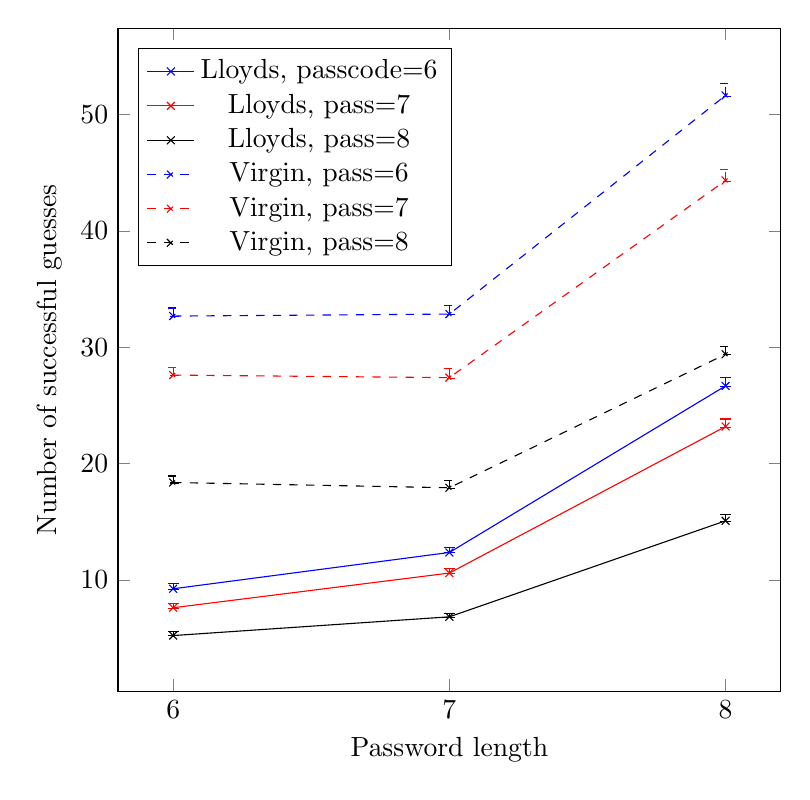
\begin{tikzpicture}
		    \begin{axis}[
		    	height=10cm,
		    	width=10cm,
		    	xtick={6,7,8},
		 xlabel=Password length,
		 ylabel=Number of successful guesses,
		 legend pos=north west
		    ]
		    \addplot[
		 mark=x,
		 blue,
		 error bars/.cd, y dir=both, y explicit,
		    ] plot coordinates {
		 (6,9.25)   -=(0,0.033) += (0,0.438)
		 (7,12.37)  -=(0,0.034) += (0,0.450)
		 (8,26.68)  -=(0,0.058) += (0,0.759)
		    };
		    \addlegendentry{Lloyds, passcode=6}

		    \addplot[
		 mark=x,
		 red,
		 error bars/.cd, y dir=both, y explicit,
		    ] plot coordinates {
		 (6,7.62)  -= (0,0.030) += (0,0.398)
		 (7,10.60) -= (0,0.030) += (0,0.397)
		 (8,23.19) -= (0,0.049) += (0,0.645)
		    };
		    \addlegendentry{Lloyds, pass=7}    

		    \addplot[
		 mark=x,
		 error bars/.cd, y dir=both, y explicit,
		    ] plot coordinates {
		 (6,5.23)  -= (0,0.025) += (0,0.329)
		 (7,6.84)  -= (0,0.024) += (0,0.319)
		 (8,15.09) -= (0,0.039) += (0,0.504)
		    };
		    \addlegendentry{Lloyds, pass=8}

		    \addplot[
		 mark=x,
		 blue,
		 dashed,
		 error bars/.cd, y dir=both, y explicit,
		    ] plot coordinates {
		 (6,32.68)  -=(0,0.053) += (0,0.695)
		 (7,32.85)  -=(0,0.058) += (0,0.753)
		 (8,51.64)  -=(0,0.078) += (0,1.026)
		    };
		    \addlegendentry{Virgin, pass=6}

		    \addplot[
		 mark=x,
		 red,
		 dashed,
		 error bars/.cd, y dir=both, y explicit,
		    ] plot coordinates {
		 (6,27.61) -= (0,0.053) += (0,0.690)
		 (7,27.39) -= (0,0.057) += (0,0.749)
		 (8,44.33) -= (0,0.070) += (0,0.921)
		    };
		    \addlegendentry{Virgin, pass=7}    

		    \addplot[
		 mark=x,
		 dashed,
		 error bars/.cd, y dir=both, y explicit,
		    ] plot coordinates {
		 (6,18.38)  -= (0,0.043) += (0,0.559)
		 (7,17.93)  -= (0,0.046) += (0,0.599)
		 (8,29.40)  -= (0,0.049) += (0,0.645)
		    };
		    \addlegendentry{Virgin, pass=8}

		    \end{axis}
		\end{tikzpicture}
		\caption{Mean number of successful guesses from ($50 \times 10^6 $) attempts using varying passcode length}
		\label{fig:approach_comparison}
	\end{figure}
	\begin{figure}[!htb]
		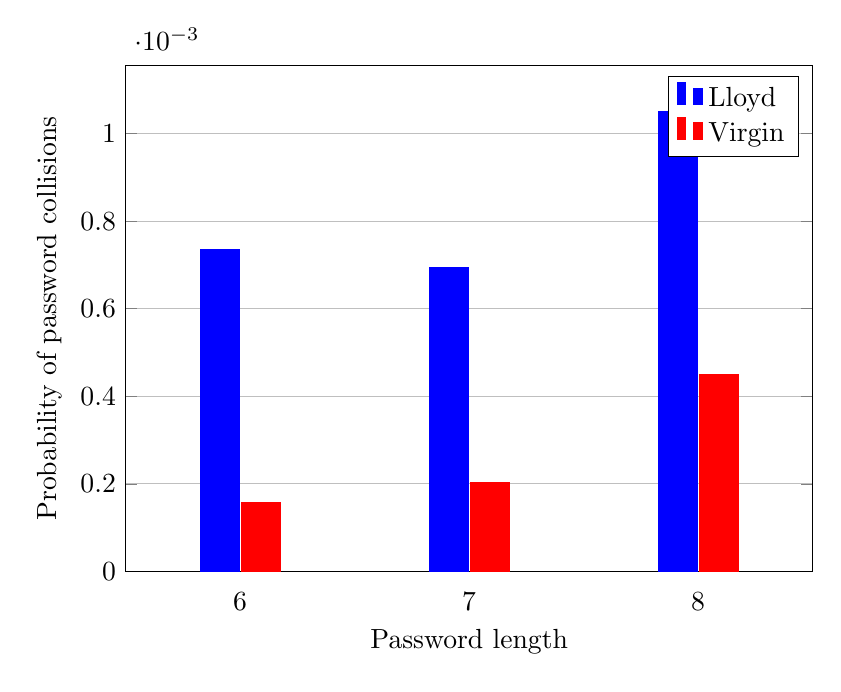
\begin{tikzpicture}
		    \begin{axis}[
		 width  = 0.85*\textwidth,
		 height = 8cm,
		 major x tick style = transparent,
		 ybar=2*\pgflinewidth,
		 bar width=14pt,
		 ymajorgrids = true,
		 ylabel = {Probability of password collisions},
		 symbolic x coords={6, 7, 8},
		 xtick = data,
		 xlabel = Password length,
		 enlarge x limits=0.25,
		 ymin=0,
		 legend cell align=left,
		    ]
		 \addplot[style={blue,fill=blue,mark=none}]
		    coordinates {(6, 7.36E-04) (7,6.94E-04) (8,1.05E-03)};

		 \addplot[style={red,fill=red,mark=none}]
		     coordinates {(6,1.56E-04) (7,2.02E-04) (8,4.50E-04)};
		 \legend{Lloyd, Virgin}
		    \end{axis}
		\end{tikzpicture}
		\caption{Probability of guessing a password using character sampled authentication (Virgin) and full password authentication (LLoyd).}
		\label{fig:collision_prob}
	\end{figure}

	\begin{figure}[!htb]
		\begin{tikzpicture}
		    \begin{axis}[ybar, xtick = {6,7,8}, xlabel = Minimum password length, ylabel = Number of valid account passwords in \cite{Cubrilovic2009-wu}]
			\addplot table [
			 col sep=comma,
			 x=pass_size,
			 y=num_pass,
			    ] {data/password_count.csv};
		    \end{axis}	    
		    \begin{axis}[
		    	axis y line*=right,
	    		axis x line=none, 
	    		ylabel = Number of valid attack passwords out of 500]
			\addplot table [
			 col sep=comma,
			 x=pass_size,
			 y=guess_pass,
			    ] {data/password_count.csv};
		    \end{axis}
		\end{tikzpicture}
		\caption{Count of valid passwords in \cite{Cubrilovic2009-wu} for each password policy}
		\label{fig:passwords_length}
	\end{figure}
	\clearpage

	\section{Main.py}\label{app:main}
	\lstinputlisting[language=Python]{../main.py}	

	\section{Statistics}\label{app:extra_stats}
	\subsection{Compiled statistics}
	\begin{table}[!htb]
		\centering
		\begin{tabular}{|l|l|l|l|l|l|l|l|}
		\hline
		& & \multicolumn{6}{l|}{\textbf{Auth system and passcode length}} \\ \hline
		\textbf{Mean} & \textbf{Password len} & \textbf{Lloyds, 6} & \textbf{Lloyds, 7} & \textbf{Lloyds, 8} & \textbf{Virgin, 6} & \textbf{Virgin, 7} & \textbf{Virgin, 8} \\ \hline
		 & 6 & 9.25 & 7.62 & 5.23 & 32.68 & 27.61 & 18.38 \\ \hline
		 & 7 & 12.37 & 10.60 & 6.84 & 32.85 & 27.39 & 17.93 \\ \hline
		 & 8 & 26.68 & 23.19 & 15.09 & 51.64 & 44.33 & 29.40 \\ \hline
		\textbf{Median} &  &  &  &  &  &  &  \\ \hline
		 & 6 & 9.00 & 7.00 & 5.00 & 33.00 & 28.00 & 18.00 \\ \hline
		 & 7 & 12.00 & 10.50 & 6.50 & 33.00 & 28.00 & 18.00 \\ \hline
		 & 8 & 27.00 & 23.00 & 15.00 & 52.00 & 44.50 & 29.00 \\ \hline
		\textbf{STD} &  &  &  &  &  &  &  \\ \hline
		 & 6 & 3.26 & 2.96 & 2.45 & 5.17 & 5.14 & 4.16 \\ \hline
		 & 7 & 3.35 & 2.95 & 2.38 & 5.61 & 5.58 & 4.46 \\ \hline
		 & 8 & 5.65 & 4.80 & 3.75 & 7.64 & 6.86 & 4.80 \\ \hline
		\textbf{Min} &  &  &  &  &  &  &  \\ \hline
		 & 6 & 2.00 & 2.00 & 1.00 & 21.00 & 16.00 & 9.00 \\ \hline
		 & 7 & 5.00 & 4.00 & 2.00 & 21.00 & 10.00 & 6.00 \\ \hline
		 & 8 & 12.00 & 11.00 & 3.00 & 32.00 & 27.00 & 20.00 \\ \hline
		\textbf{Max} &  &  &  &  &  &  &  \\ \hline
		 & 6 & 18.00 & 15.00 & 14.00 & 46.00 & 43.00 & 29.00 \\ \hline
		 & 7 & 21.00 & 20.00 & 13.00 & 48.00 & 43.00 & 31.00 \\ \hline
		 & 8 & 43.00 & 38.00 & 24.00 & 75.00 & 64.00 & 44.00 \\ \hline
		\textbf{0.1 confi.} &  &  &  &  &  &  &  \\ \hline
		 & 6 & 0.033 & 0.030 & 0.025 & 0.053 & 0.053 & 0.043 \\ \hline
		 & 7 & 0.034 & 0.030 & 0.024 & 0.058 & 0.057 & 0.046 \\ \hline
		 & 8 & 0.058 & 0.049 & 0.039 & 0.078 & 0.070 & 0.049 \\ \hline
		\textbf{0.9 confi.} &  &  &  &  &  &  &  \\ \hline
		 & 6 & 0.438 & 0.398 & 0.329 & 0.695 & 0.690 & 0.559 \\ \hline
		 & 7 & 0.450 & 0.397 & 0.319 & 0.753 & 0.749 & 0.599 \\ \hline
		 & 8 & 0.759 & 0.645 & 0.504 & 1.026 & 0.921 & 0.645 \\ \hline
		\end{tabular}
		\caption{Individual statistics for each authentication system and password/passcode length combination}
	\end{table}
	\clearpage

  	\subsection{Data significance}
  	\label{app:significant_stats}
  	The following table details the results of statistical tests between each authentication system using equivalent password/passcode length policies.
  	\begin{table}[!htb]
	\centering
	\begin{tabular}{|p{2cm}|l|l|l|l|}
	\hline
	\textbf{Password/ Passcode length} & \textbf{Lloyds median} & \textbf{Virgin median} & \textbf{Mann whitney Z-score} & \textbf{p value} \\ \hline
	6,6 & 9 & 33 & -14.974 & p\textless0.01 \\ \hline
	6,7 & 7 & 27.5 & -14.974 & p\textless0.01 \\ \hline
	6,8 & 5 & 18 & -15.100 & p\textless0.01 \\ \hline
	7,6 & 12 & 33 & -14.974 & p\textless0.01 \\ \hline
	7,7 & 10.5 & 28 & -14.793 & p\textless0.01 \\ \hline
	7,8 & 6.5 & 18 & -14.596 & p\textless0.01 \\ \hline
	8,6 & 27 & 52 & -14.898 & p\textless0.01 \\ \hline
	8,7 & 23 & 44.5 & -14.801 & p\textless0.01 \\ \hline
	8,8 & 15 & 29 & -14.794 & p\textless0.01 \\ \hline
	\end{tabular}
	\caption{Statistical tests between authentication systems for equivalent password/passcode length}
	\label{tab:significance}
	\end{table}
	\clearpage
	\subsection{Sample of raw data}
	\label{app:raw_data}
	\begin{longtable}{|p{0.5cm}|p{0.5cm}|p{0.5cm}|p{0.5cm}|p{0.5cm}|p{0.5cm}|p{0.5cm}|p{0.5cm}|p{0.5cm}|p{0.5cm}|p{0.5cm}|p{0.5cm}|p{0.5cm}|p{0.5cm}|p{0.5cm}|p{0.5cm}|p{0.5cm}|p{0.5cm}|}
	\hline
	\multicolumn{18}{|l|}{\textbf{Password/Passcode policy in format N1/N2, Lloyds $\rightarrow$ full, Virgin $\rightarrow$ Virgin}} \\ \hline
	\multicolumn{2}{|l|}{\textbf{6,6}} & \multicolumn{2}{l|}{\textbf{6,7}} & \multicolumn{2}{l|}{\textbf{6,8}} & \multicolumn{2}{l|}{\textbf{7,6}} & \multicolumn{2}{l|}{\textbf{7,7}} & \multicolumn{2}{l|}{\textbf{7,8}} & \multicolumn{2}{l|}{\textbf{8,6}} & \multicolumn{2}{l|}{\textbf{8,7}} & \multicolumn{2}{l|}{\textbf{8,8}} \\ \hline
	LLo & Virg & LLo & Virg & LLo & Virg & LLo & Virg & LLo & Virg & LLo & Virg & LLo & Virg & LLo & Virg & LLo & Virg \\ \hline
	12 & 36 & 6 & 27 & 3 & 24 & 7 & 23 & 10 & 21 & 6 & 17 & 21 & 42 & 32 & 51 & 16 & 26 \\ \hline
	17 & 39 & 12 & 28 & 7 & 17 & 14 & 48 & 13 & 26 & 6 & 19 & 29 & 47 & 23 & 37 & 16 & 30 \\ \hline
	11 & 27 & 5 & 23 & 5 & 11 & 13 & 42 & 13 & 26 & 5 & 11 & 31 & 57 & 20 & 46 & 18 & 35 \\ \hline
	11 & 32 & 7 & 29 & 3 & 17 & 8 & 32 & 5 & 20 & 7 & 21 & 24 & 47 & 20 & 42 & 13 & 26 \\ \hline
	9 & 21 & 7 & 26 & 5 & 17 & 7 & 28 & 10 & 27 & 7 & 13 & 27 & 52 & 28 & 48 & 11 & 29 \\ \hline
	13 & 42 & 11 & 27 & 2 & 14 & 14 & 45 & 11 & 25 & 4 & 18 & 24 & 57 & 16 & 30 & 9 & 24 \\ \hline
	12 & 36 & 4 & 23 & 4 & 15 & 12 & 36 & 8 & 31 & 5 & 21 & 29 & 58 & 24 & 44 & 17 & 33 \\ \hline
	13 & 36 & 11 & 35 & 4 & 14 & 10 & 27 & 11 & 27 & 7 & 15 & 40 & 64 & 31 & 62 & 19 & 34 \\ \hline
	10 & 40 & 12 & 39 & 7 & 21 & 6 & 25 & 12 & 30 & 4 & 18 & 30 & 54 & 25 & 48 & 15 & 34 \\ \hline
	10 & 34 & 8 & 22 & 6 & 17 & 16 & 34 & 11 & 32 & 3 & 11 & 37 & 59 & 21 & 38 & 15 & 28 \\ \hline
	5 & 32 & 7 & 28 & 5 & 14 & 19 & 29 & 13 & 26 & 5 & 17 & 29 & 49 & 15 & 34 & 13 & 32 \\ \hline
	17 & 34 & 4 & 26 & 3 & 19 & 11 & 29 & 12 & 30 & 4 & 16 & 20 & 43 & 19 & 40 & 22 & 34 \\ \hline
	5 & 26 & 9 & 30 & 7 & 18 & 14 & 42 & 10 & 21 & 10 & 17 & 33 & 67 & 21 & 43 & 20 & 30 \\ \hline
	16 & 30 & 5 & 26 & 3 & 13 & 16 & 33 & 12 & 29 & 6 & 20 & 31 & 65 & 20 & 51 & 17 & 22 \\ \hline
	18 & 46 & 8 & 23 & 5 & 25 & 15 & 36 & 18 & 36 & 12 & 20 & 29 & 46 & 24 & 44 & 22 & 31 \\ \hline
	15 & 39 & 3 & 27 & 8 & 27 & 10 & 28 & 11 & 23 & 6 & 22 & 31 & 67 & 20 & 39 & 17 & 29 \\ \hline
	10 & 37 & 7 & 29 & 5 & 21 & 17 & 43 & 11 & 28 & 6 & 11 & 19 & 47 & 27 & 48 & 19 & 35 \\ \hline
	8 & 30 & 5 & 21 & 3 & 13 & 11 & 31 & 11 & 24 & 8 & 17 & 21 & 44 & 26 & 50 & 12 & 22 \\ \hline
	9 & 33 & 3 & 23 & 3 & 14 & 9 & 28 & 13 & 23 & 12 & 23 & 23 & 44 & 18 & 40 & 19 & 36 \\ \hline
	... & ... & ...& ... & ...& ... & ...& ... & ... & ... & ...& ... & ... & ... & ... & ... & ... & ... \\ \hline
		\caption{Raw data, displaying the number of successful matches in each authentication using 50 million guesses of attack \& victim password/passcodes. 150 data points exist in each password / passcode policy and authentication system, the full table can be found in data/raw\_data.csv}
	\label{tab:raw_data}
	\end{longtable}

	\clearpage

	\section{BruteForce.py}\label{app:bruteforce}
	\lstinputlisting[language=Python]{../bruteforce.py}

	\section{Brute force results}\label{app:bruteforceresults}
	\begin{table}[h]
	\centering
	\begin{tabular}{l|l|l|l|l|l|l|}
	\cline{2-7}
	 & \multicolumn{3}{l|}{\textbf{Partial matching}} & \multicolumn{3}{l|}{\textbf{Full password matching}} \\ \cline{2-7} 
	 & \textit{Successful guesses} & \textit{Attempts} & \textit{Success ratio} & \multicolumn{3}{l|}{\textit{Successful guesses}} \\ \hline
	\multicolumn{1}{|l|}{\textbf{6}} & 1.49E+08 & 2.02E+11 & 7.36E-04 & 1.58E+06 & 1.01E+10 & 1.56E-04 \\ \hline
	\multicolumn{1}{|l|}{\textbf{7}} & 6.70E+07 & 9.66E+10 & 6.94E-04 & 5.57E+05 & 2.76E+09 & 2.02E-04 \\ \hline
	\multicolumn{1}{|l|}{\textbf{8}} & 3.77E+07 & 3.57E+10 & 1.05E-03 & 2.87E+05 & 6.37E+08 & 4.50E-04 \\ \hline
	\end{tabular}
	\caption{Number of successful matches for every permutation of attack/victim passwords, weighed in function of the number of users using that password.}
	\label{tab:brute_force}
	\end{table}

\end{appendices}
\clearpage
\end{document}
